\documentclass[12pt]{article}
\usepackage{amsmath,amssymb,amsthm}
\usepackage{fullpage}
\usepackage{graphicx}
\usepackage{hyperref}

\theoremstyle{definition}
\newtheorem{thm}{Theorem}[section]
\newtheorem{lem}[thm]{Lemma}
\newtheorem{defn}{Definition}[section]
\newcommand{\floor}[1]{\left\lfloor #1 \right\rfloor}
\newcommand{\ceil}[1]{\left\lceil #1 \right\rceil}
\newcommand{\bigC}[0]{\mathcal{C}}
\begin{document}
\title{
An attempt to connect Shannon's
circuit counting bound with clique detection}

\author{Josh Burdick \\
Howard Hughes Medical Institute \\
{\tt josh.t.burdick@gmail.com}}
\maketitle

\begin{abstract}
Shannon's function-counting argument
\cite{shannon_synthesis_1949} showed that some Boolean functions have
exponential circuit complexity, but doesn't provide a specific example
of such a hard-to-compute function. A simple modification of that argument
shows that detecting a randomly-chosen subset of the $k$-vertex cliques in an
$n$-vertex graph requires, on average, $\Omega(n^{k/2})$ NAND gates.
Unfortunately,
this doesn't directly bound the complexity of detecting {\em all} of the cliques; however, it seems like a
possibly related problem.
Here, we attempt to connect this
average-case bound on detecting some
cliques, with the problem of detecting all of them.
\end{abstract}

\newpage

\tableofcontents

\section{A counting bound}
\label{countingBound}

The first component we use is a slight modification
of Shannon's function-counting argument
\cite{shannon_synthesis_1949}.

\subsection{Background: lower bounds from function counting}

It has long been known that computing {\em some} function of a bit-string
requires exponentially large circuits \cite{shannon_synthesis_1949}.
If there are $m$ inputs to a circuit,
then there are $2^{2^m}$ possible functions from the $m$-input bitstring to
a one-bit output. Each of these functions, being different, must have a
different circuit.

Let $\bigC(f)$ be the circuit
with the fewest unbounded fan-in NAND
gates computing $f$ (with ties broken
arbitrarily). 

If we assume the circuit is made of NAND gates, and has $g$ gates, then the
circuit could have at most $gm$ wires from inputs to gates, and ${g \choose 2}$
wires from gates to gates. We can view the possible circuits as a bitmask,
containing a 1 everywhere a gate is connected to an input (or another gate),
and 0 everywhere else.

\begin{thm}
\label{boundFromCounting}
Consider functions from $m$ bits to one bit of output.
This means that, with $g$ gates, we can represent at most
$2^{gm + {g \choose 2}}$ different boolean functions (with $m$ bits of input,
and one bit of output).
\end{thm}
\begin{proof}

The number of possible wires which are there, or not, is $gm + {g \choose 2}$,
which bounds how many possible circuits there are.
Some of these circuits compute the same function.
However, there can't be any more than this many circuits with this many wires.
\end{proof}

This means that if we have a large set of functions, and we know the size of
the set of functions, then we know that at least {\em one} of them requires
a large number of gates. (Knowing {\em which} function requires a lot, or many,
gates is still an issue).

Consider functions from $m$ bits to one bit of output.
Let $g$ be the number of gates, and $w$ be the number of wires.
Solving for the number of gates:

\begin{eqnarray*}
w & = & mg + {g \choose 2} \\
  & = & mg + g(g-1)/2 \\
  & = & mg + (g^2 - g) / 2 \\
  & = & 0.5g^2 + (m-0.5)g \\
0 & = & 0.5g^2 + (m-0.5)g - w \\
\end{eqnarray*}

We solve the quadratic formula (writing $b = m-0.5$ for simplicity), keeping
only the non-imaginary root.

\begin{eqnarray*}
g & = & -b \pm \sqrt{ b^2 + 2w} \\
  & = & {\sqrt {2w + b^2}} - b \\
\end{eqnarray*}

Thus, given a set of functions, we know that at least one of them requires
some number of gates.

\subsection{Bounding the average number of gates}

We can also count the total number of functions from $m$ input bits to one
output bit, using up to $g$ NAND gates, as

\begin{eqnarray*}
\sum_{i=0}^{g-1} 2^{m+i} & = & 2^{m+g} - 2^m
\end{eqnarray*}

If we're counting circuits with up to $g$ gates, then some of the circuits
have fewer than $g$ gates. This somewhat complicates the book-keeping.
However, {\em most} of the
circuits have $g$ gates. (Indeed, well over half, since each additional
gate adds many potential wires). Because of this, I think that the
average case bound is just one fewer gates than the worst-case bound.

\subsection{Counting CLIQUE-like functions}

We now consider ``buggy'' NAND gate circuits (with any fan-in) which find some of the possible $k$-cliques in $n$-vertex
graphs.
For concreteness,
consider a set of ``buggy'' 6-clique finders. 
Maybe the circuit correctly
finds all the cliques. Or maybe it finds all of the cliques except $K_{1..6}$,
or it misses half the cliques, or finds none (and always outputs 0), or maybe
it only successfully finds $K_{1,3,4,5,7,8}$, et cetera. More formally
(and generally),
we define a set of functions ({\em not} circuits):


\begin{defn}
\label{BUGGY-k-CLIQUE}
BUGGY-$k$-CLIQUE$(n)$ is the set of functions which recognize any set
of $K_k$s. That is, for each set $A$ of $K_k$s, BUGGY-$k$-CLIQUE$(n)$
contains a function which is 1 if the input contains any $K_6 \in A$,
and 0 otherwise.
\end{defn}

This clearly includes $k$-CLIQUE (which finds all the cliques).

These functions are all distinct. If $f_1,f_2\in $BUGGY-$k$-CLIQUE$(n)$,
then there's some $K_k$ such that if $y$ is the graph with {\em only}
1's in that $K_k$ (and 0's elsewhere), $f_1(y) = 0$ and $f_2(y) = 1$.

Of course, many of these functions are quite similar (e.g. all but one of them
output a 1 when you feed in all 1's). However, they're all slightly different.

\begin{thm}
\label{buggyDistinct}
BUGGY-$k$-CLIQUE$(n)$ contains $2^{n \choose k}$ distinct functions.
\end{thm}
\begin{proof}
That is how many subsets of the $K_k$s there are.
\end{proof}

Although $2^{n \choose k}$ is a fairly large number,
it's still comfortably less than $2^{2^{n \choose 2}}$, the number of boolean
functions on the ${n \choose 2}$ input wires (one per edge).

\subsubsection{But {\em which} function requires many gates?}

Thus, there are $2^{n \choose k}$ different functions. 
How many NAND gates do these take?
(We consider NAND gate circuits (with any fan-in) which find $k$-cliques in $n$-vertex
graphs, as a circuit with $n \choose 2$ inputs)

Applying Theorem
\ref{boundFromCounting}, we know that at least one of the circuits requires
${\sqrt {2 {n \choose {k/2}} + b^2}} - b = \Omega(n^{k/2})$ 
NAND gates (where $b = {k \choose 2} - 0.5$).

Why doesn't this bound HAS-$k$-CLIQUE?
Because we don't know that the circuit which finds {\em all} of the
$K_k$s, is one of these larger circuits. As far as what I've
shown thus far goes, it could be harder to find some weird subset of the $K_k$s.

Indeed, as far as what I've formally shown goes, the problem which needs
the most NAND gates could be finding a single $K_k$! That's easily ruled out
(because that only needs one NAND gate, plus the output gate).

\subsection{Which sets of cliques are hard to find?}
\label{sec:whichCliques}

The hardness of these functions depends
on how the cliques they find are laid out.

Cliques are arguably difficult to draw in a two-dimensional space.
As an approximate diagram reflecting what we know,
we sketch a Hasse of possible subsets of cliques. Although
we only draw a few subsets of three-vertex cliques
on six vertices, hopefully this provides some
intuition.

\begin{figure}
\centering
\includegraphics[width=1\textwidth]{R/Hasse.pdf}
\caption{Hasse diagram of circuits}
\label{fig:Hasse}
\end{figure}



\begin{thm}
\label{edgeZonking}
Suppose a circuit finds 
\end{thm}
\begin{proof}
Suppose we feed in
\end{proof}

This shows that finding many subsets of cliques is harder than
many smaller subsets of cliques. This suggests that in general,
finding more cliques requires more gates, but doesn't prove it.


Triangles can be detected using matrix multiplication \cite{itai_finding_1977},
and there are fast algorithms known for matrix multiplication
\cite{strassen_gaussian_1969}
\cite{williams_multiplying_2012}, so
the triangles on the left can be detected
using fewer than one NAND gate per triangle (for large enough input graphs).

On the other hand, if the triangles overlap less (as on the right),
then to detect all of the triangles, we will definitely need at least one
gate per triangle.
To see this, consider feeding in a 0 to the input for one
of the edges unique to some triangle (this is a
standard technique in circuit bounds).
Then any gate connected to
that edge will only output a constant 1. We can repeat this for each of the
triangles, constructing a series of strictly smaller circuits, each of which 

It seems intuitive that, in some sense, finding more cliques should
be harder.
Indeed, since we're using NAND gates, we know that finding any non-empty
subset of cliques is strictly harder than finding {\em some} other 
smaller set of cliques (namely, the set you get after feeding in 0's to
all the edges connected to some vertex).
Unfortunately, the relevance of this to the difficulty
of $k$-CLIQUE is not clear.

\section{Counting slightly larger sets of functions}


We construct somewhat larger sets of functions, based on
which cliques they recognize. For instance, we can define the
function PICKY-CLIQUE.


\begin{defn}{pickyClique}
Let $A$ be a set of cliques, and $B \subset A$.
Define PICKY-CLIQUE(A, B) to be the function which is 1 iff

\begin{itemize}

\item any clique in $A-B$ is present, {\em and}

\item no clique in $B$ is present

\end{itemize}
Cliques outside of $A$ are ignored.

\end{defn}




We can also construct somewhat larger sets of functions. For instance,
suppose that, rather than detecting or ignoring each clique, we assign
to each clique either 1, 0, or X, with this interpretation:

\begin{itemize}

\item 1: ``If any of these cliques is present, then output 1...''

\item 0: ``...unless one of these cliques is present, in which case output 0.''

\item X: ``(Ignore whether this clique is present).''

\end{itemize}

There are $3^{n \choose k}$ such strings. However, those consisting only of
0's and X's always output 0, and so are indistinguishable, so there are
only $3^{n \choose k} - 2^{n \choose k}$ distinct functions.

The lower bound on the average hardness of computing these functions is
slightly higher. However, this doesn't seem to help that much.

Note that distinguishing the functions requires that we be able to have at
least two distinct cliques either be present or absent. With two cliques,
we can do this by feeding in 1's to any edges shared by the cliques, and
then feeding in 0's or 1's to the remaining edges:

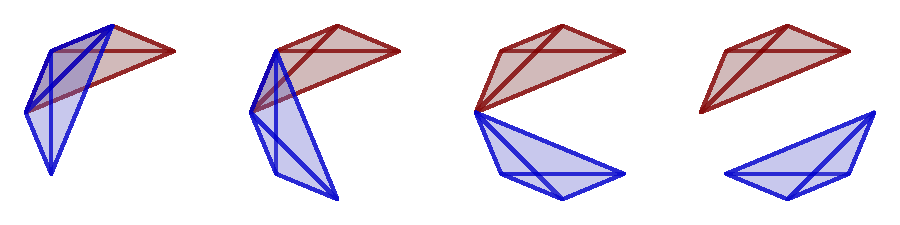
\includegraphics[width=0.7\textwidth]{R/overlapping.pdf}

However, it seems hard to push this to arbitrary functions of ``which cliques are
present'', because they start to overlap.





\section{Related work}

This strategy relies heavily on a modification of Shannon's original
function-counting argument \cite{shannon_synthesis_1949}.

Broadly speaking, the idea of using an upper bound to prove a lower bound
is not new. Aaronson describes this as ``ironic complexity theory''
\cite{aaronson_pnp}, and mentions several recent applications of it.

\subsection{Possible relevance to other problems}

Here we sketch other potential applications of this strategy.

\subsubsection{The complement of NP: co-NP}

FIXME is this right?

Although there's no obvious reduction from co-NP to NP, essentially
the same argument seems to work. Suppose some family of circuits
checks that there {\em isn't} any $K_k$ in an $n$-vertex graph.
Then we can check that an arbitrary graph is free of $K_k$s by
ANDing together circuits which check that subsets of vertices are
clear of $K_k$s. (ANDing them all together can be done with
two additional NAND gates; there may be a cheaper way).

\subsubsection{Quantum computation: BQP}

This lower-bound strategy also seems potentially
relevant to quantum computing,
as the argument makes few restrictions on the sort of gates used.
If it's the case that any function in BQP can be represented
as a circuit made of discrete quantum gates, as well as AND and NOT,
then clique detection isn't in BQP.
However, it's not clear what sort of quantum gates would be
appropriate.

\section{Conclusion}

We give a lower bound on finding {\em some} set of cliques.
It is a modified form of Shannon's counting argument
\cite{shannon_synthesis_1949}. Unfortunately,
this doesn't seem directly related to the
complexity of 

\section{Acknowledgements}

The author would like to thank William Gasarch for introducing him
to lower bound strategies and probabilistic proofs about graphs. He would
also like to thank the Cheung lab for
employment, and his parents for financial support.

\bibliography{references}
\bibliographystyle{abbrv}

\end{document}

